\documentclass[12pt,a4paper]{article}
\usepackage[utf8]{inputenc}
\usepackage{amsmath}
\usepackage{amsfonts}
\usepackage{amssymb}
\usepackage{graphicx}
\usepackage{listings}
\author{Imelda Finn}
\title{Analysis of Midwest Poverty}
\begin{document}
	\maketitle
	
\section*{Introduction}
%Midwest demographics
Description
Demographic information of midwest counties from 2000 US census

Usage
midwest
Format
A data frame with 437 rows and 28 variables:


\begin{enumerate}

\item PID
Unique county identifier.

\item county
County name.

\item state
State to which county belongs to.

\item area
Area of county (units unknown).

\item poptotal
Total population.

\item popdensity
Population density (person/unit area).

\item popwhite
Number of whites.

\item popblack
Number of blacks.

\item popamerindian
Number of American Indians.

\item popasian
Number of Asians.

\item popother
Number of other races.

\item percwhite
Percent white.

\item percblack
Percent black.

\item percamerindan
Percent American Indian.

\item percasian
Percent Asian.

\item percother
Percent other races.

\item popadults
Number of adults.

\item perchsd
Percent with high school diploma.

\item percollege
Percent college educated.

\item percprof
Percent with professional degree.

\item poppovertyknown
Population with known poverty status.

\item percpovertyknown
Percent of population with known poverty status.

\item percbelowpoverty
Percent of people below poverty line.

\item percchildbelowpovert
Percent of children below poverty line.

\item percadultpoverty
Percent of adults below poverty line.

\item percelderlypoverty
Percent of elderly below poverty line.

\item inmetro
County considered in a metro area.

\item category
Miscellaneous.

\end{enumerate}



\section*{Research Question}

\section*{Analysis}
\begin{figure}[h!]\centering
	\caption{\footnotesize Facet Wrap}
	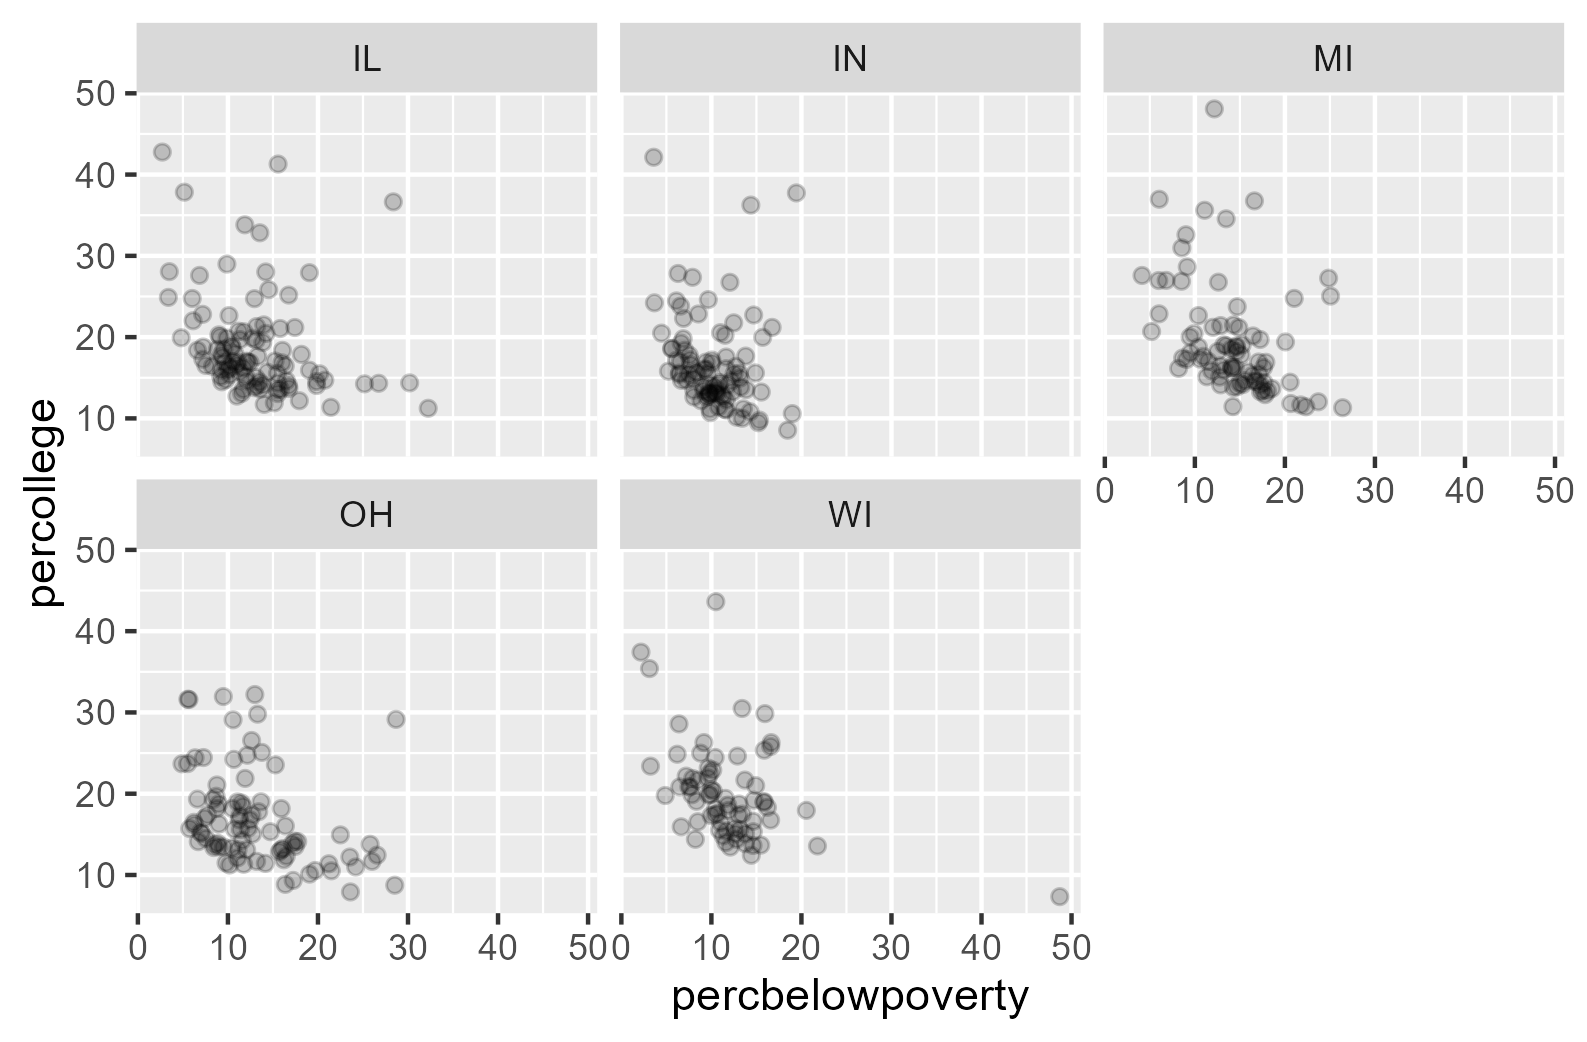
\includegraphics[width=.75\textwidth]{facet_wrap.png}
\end{figure} 

\section*{Conclusion}

\end{document}